\documentclass{standalone}
\usepackage{tikz}
\usetikzlibrary{patterns, positioning}
\usepackage[sfdefault]{ClearSans} %% option 'sfdefault' activates Clear Sans as the default text font
\usepackage[T1]{fontenc}

\begin{document}
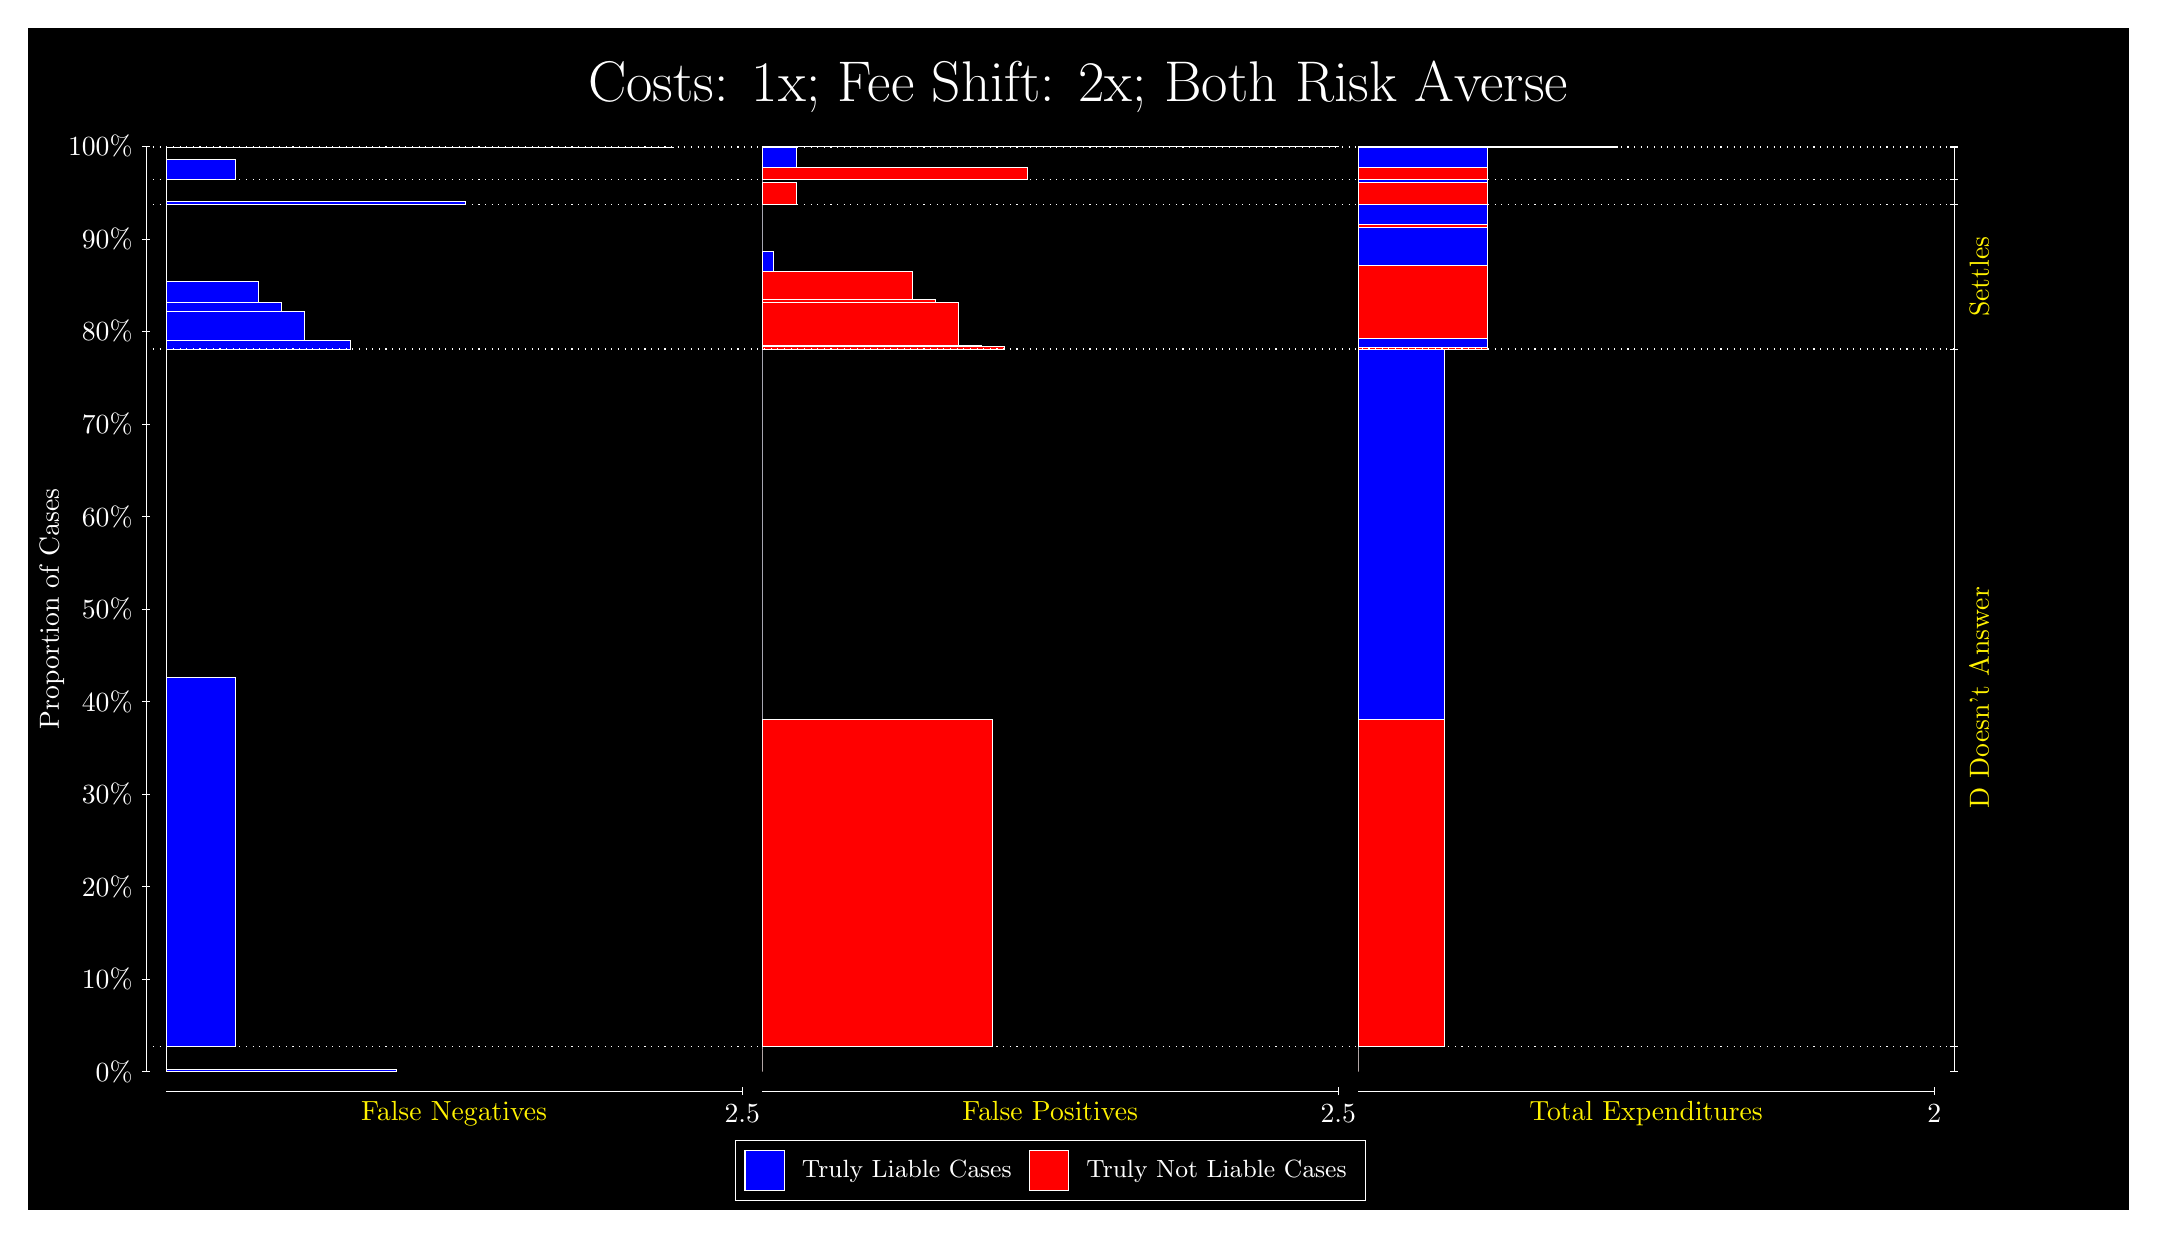
\begin{tikzpicture}
\draw[fill=black] (0,0) rectangle (26.667,15);
\draw[text=white] (0,13.5) rectangle (26.667,15) node[midway] {\huge Costs: 1x; Fee Shift: 2x; Both Risk Averse};
\draw[white, very thin] (1.5,1.75) -- (1.5,13.5);
\node[rotate=90, text=white, anchor=center] at (0.3, 7.625) {Proportion of Cases};
\draw[white, very thin] (1.45,1.75) -- (1.55,1.75);
\node[text=white, anchor=east] at (1.45, 1.75) {0\%};
\draw[white, very thin] (1.45,2.925) -- (1.55,2.925);
\node[text=white, anchor=east] at (1.45, 2.925) {10\%};
\draw[white, very thin] (1.45,4.1) -- (1.55,4.1);
\node[text=white, anchor=east] at (1.45, 4.1) {20\%};
\draw[white, very thin] (1.45,5.275) -- (1.55,5.275);
\node[text=white, anchor=east] at (1.45, 5.275) {30\%};
\draw[white, very thin] (1.45,6.45) -- (1.55,6.45);
\node[text=white, anchor=east] at (1.45, 6.45) {40\%};
\draw[white, very thin] (1.45,7.625) -- (1.55,7.625);
\node[text=white, anchor=east] at (1.45, 7.625) {50\%};
\draw[white, very thin] (1.45,8.8) -- (1.55,8.8);
\node[text=white, anchor=east] at (1.45, 8.8) {60\%};
\draw[white, very thin] (1.45,9.975) -- (1.55,9.975);
\node[text=white, anchor=east] at (1.45, 9.975) {70\%};
\draw[white, very thin] (1.45,11.15) -- (1.55,11.15);
\node[text=white, anchor=east] at (1.45, 11.15) {80\%};
\draw[white, very thin] (1.45,12.325) -- (1.55,12.325);
\node[text=white, anchor=east] at (1.45, 12.325) {90\%};
\draw[white, very thin] (1.45,13.5) -- (1.55,13.5);
\node[text=white, anchor=east] at (1.45, 13.5) {100\%};

\draw[white, very thin] (24.457,1.75) -- (24.457,13.5);
\draw[white, very thin] (24.407,1.75) -- (24.507,1.75);
\node[anchor=west] at (24.407, 1.75) {};
\draw[white, very thin] (24.407,2.0652) -- (24.507,2.0652);
\node[anchor=west] at (24.407, 2.0652) {};
\draw[white, very thin] (24.407,10.926) -- (24.507,10.926);
\node[anchor=west] at (24.407, 10.926) {};
\draw[white, very thin] (24.407,12.761) -- (24.507,12.761);
\node[anchor=west] at (24.407, 12.761) {};
\draw[white, very thin] (24.407,13.079) -- (24.507,13.079);
\node[anchor=west] at (24.407, 13.079) {};
\draw[white, very thin] (24.407,13.487) -- (24.507,13.487);
\node[anchor=west] at (24.407, 13.487) {};
\draw[white, very thin] (24.407,13.496) -- (24.507,13.496);
\node[anchor=west] at (24.407, 13.496) {};
\draw[white, very thin] (24.407,13.5) -- (24.507,13.5);
\node[anchor=west] at (24.407, 13.5) {};

\draw[white, very thin, fill=blue] (1.75,1.75) rectangle (4.6775,1.7832);
\draw[white, very thin, fill=red] (1.75,1.7832) rectangle (1.75,2.0652);
\draw[white, very thin, fill=blue] (1.75,2.0652) rectangle (2.6283,6.7621);
\draw[white, very thin, fill=red] (1.75,6.7621) rectangle (1.75,10.926);
\draw[white, very thin, fill=blue] (1.75,10.926) rectangle (4.092,11.033);
\draw[white, very thin, fill=blue] (1.75,11.033) rectangle (3.7993,11.038);
\draw[white, very thin, fill=blue] (1.75,11.038) rectangle (3.5065,11.409);
\draw[white, very thin, fill=blue] (1.75,11.409) rectangle (3.2138,11.524);
\draw[white, very thin, fill=blue] (1.75,11.524) rectangle (2.921,11.78);
\draw[white, very thin, fill=red] (1.75,11.78) rectangle (1.75,12.761);
\draw[white, very thin, fill=blue] (1.75,12.761) rectangle (5.5558,12.796);
\draw[white, very thin, fill=red] (1.75,12.796) rectangle (1.75,13.079);
\draw[white, very thin, fill=blue] (1.75,13.079) rectangle (2.6283,13.33);
\draw[white, very thin, fill=red] (1.75,13.33) rectangle (1.75,13.487);
\draw[white, very thin, fill=blue] (1.75,13.487) rectangle (8.1906,13.489);
\draw[white, very thin, fill=red] (1.75,13.489) rectangle (1.75,13.496);
\draw[white, very thin, fill=red] (1.75,13.496) rectangle (1.75,13.498);
\draw[white, very thin, fill=blue] (1.75,13.498) rectangle (1.75,13.5);
\draw[white, very thin, fill=red] (9.3189,1.75) rectangle (9.3189,2.032);
\draw[white, very thin, fill=blue] (9.3189,2.032) rectangle (9.3189,2.0652);
\draw[white, very thin, fill=red] (9.3189,2.0652) rectangle (12.246,6.2293);
\draw[white, very thin, fill=blue] (9.3189,6.2293) rectangle (9.3189,10.926);
\draw[white, very thin, fill=red] (9.3189,10.926) rectangle (12.393,10.958);
\draw[white, very thin, fill=red] (9.3189,10.958) rectangle (12.1,10.975);
\draw[white, very thin, fill=red] (9.3189,10.975) rectangle (11.807,11.514);
\draw[white, very thin, fill=red] (9.3189,11.514) rectangle (11.515,11.562);
\draw[white, very thin, fill=red] (9.3189,11.562) rectangle (11.222,11.907);
\draw[white, very thin, fill=blue] (9.3189,11.907) rectangle (9.4652,12.163);
\draw[white, very thin, fill=blue] (9.3189,12.163) rectangle (9.3189,12.761);
\draw[white, very thin, fill=red] (9.3189,12.761) rectangle (9.758,13.043);
\draw[white, very thin, fill=blue] (9.3189,13.043) rectangle (9.3189,13.079);
\draw[white, very thin, fill=red] (9.3189,13.079) rectangle (12.686,13.236);
\draw[white, very thin, fill=blue] (9.3189,13.236) rectangle (9.758,13.487);
\draw[white, very thin, fill=red] (9.3189,13.487) rectangle (9.3189,13.494);
\draw[white, very thin, fill=blue] (9.3189,13.494) rectangle (9.3189,13.496);
\draw[white, very thin, fill=red] (9.3189,13.496) rectangle (16.638,13.498);
\draw[white, very thin, fill=blue] (9.3189,13.498) rectangle (13.71,13.5);
\draw[white, very thin, fill=red] (16.888,1.75) rectangle (16.888,2.032);
\draw[white, very thin, fill=blue] (16.888,2.032) rectangle (16.888,2.0652);
\draw[white, very thin, fill=red] (16.888,2.0652) rectangle (17.986,6.2293);
\draw[white, very thin, fill=blue] (16.888,6.2293) rectangle (17.986,10.926);
\draw[white, very thin, fill=red] (16.888,10.926) rectangle (18.534,10.944);
\draw[white, very thin, fill=blue] (16.888,10.944) rectangle (18.534,11.059);
\draw[white, very thin, fill=red] (16.888,11.059) rectangle (18.534,11.991);
\draw[white, very thin, fill=blue] (16.888,11.991) rectangle (18.534,12.474);
\draw[white, very thin, fill=red] (16.888,12.474) rectangle (18.534,12.505);
\draw[white, very thin, fill=blue] (16.888,12.505) rectangle (18.534,12.761);
\draw[white, very thin, fill=red] (16.888,12.761) rectangle (18.534,13.043);
\draw[white, very thin, fill=blue] (16.888,13.043) rectangle (18.534,13.079);
\draw[white, very thin, fill=red] (16.888,13.079) rectangle (18.534,13.236);
\draw[white, very thin, fill=blue] (16.888,13.236) rectangle (18.534,13.487);
\draw[white, very thin, fill=red] (16.888,13.487) rectangle (20.181,13.494);
\draw[white, very thin, fill=blue] (16.888,13.494) rectangle (20.181,13.496);
\draw[white, very thin, fill=red] (16.888,13.496) rectangle (20.181,13.498);
\draw[white, very thin, fill=blue] (16.888,13.498) rectangle (20.181,13.5);
\draw[white, dotted] (1.5,2.0652) -- (24.457,2.0652);
\draw[white, dotted] (1.5,10.926) -- (24.457,10.926);
\draw[white, dotted] (1.5,12.761) -- (24.457,12.761);
\draw[white, dotted] (1.5,13.079) -- (24.457,13.079);
\draw[white, dotted] (1.5,13.487) -- (24.457,13.487);
\draw[white, dotted] (1.5,13.496) -- (24.457,13.496);
\draw[white, very thin] (1.75,1.5) -- (9.0689,1.5);
\node[text=yellow, anchor=north] at (5.4094, 1.5) {False Negatives};
\draw[white, very thin] (9.0689,1.45) -- (9.0689,1.55);
\node[text=white, anchor=north] at (9.0689, 1.45) {2.5};

\draw[white, very thin] (9.3189,1.5) -- (16.638,1.5);
\node[text=yellow, anchor=north] at (12.978, 1.5) {False Positives};
\draw[white, very thin] (16.638,1.45) -- (16.638,1.55);
\node[text=white, anchor=north] at (16.638, 1.45) {2.5};

\draw[white, very thin] (16.888,1.5) -- (24.207,1.5);
\node[text=yellow, anchor=north] at (20.547, 1.5) {Total Expenditures};
\draw[white, very thin] (24.207,1.45) -- (24.207,1.55);
\node[text=white, anchor=north] at (24.207, 1.45) {2};


\node[text=yellow, centered, rotate=90] at (24.777, 6.4957) {D Doesn't Answer};
\node[text=yellow, centered, rotate=90] at (24.777, 11.843) {Settles};





\draw (12.978300999999998,1.5) node[draw=none] (baseCoordinate) {};
\begin{scope}[align=center]
        \matrix[scale=0.5, draw=white, below=0.5cm of baseCoordinate, nodes={draw}, column sep=0.1cm]{
            \node[rectangle, draw, minimum width=0.5cm, minimum height=0.5cm, fill=blue] {}; &
            \node[draw=none, font=\small, text=white] (B) {Truly Liable Cases}; &
            \node[rectangle, draw, minimum width=0.5cm, minimum height=0.5cm, fill=red] {}; &
            \node[draw=none, font=\small, text=white] (B) {Truly Not Liable Cases}; \\
            };
\end{scope}

\end{tikzpicture}
\end{document}